\documentclass[compress]{beamer}
\usepackage{hyperref}
\usepackage[utf8]{inputenc}
\usepackage{graphicx}
\author{Marzio De Corato}
\usepackage{varwidth}
\usepackage{beamerthemesplit} 

\usepackage[english]{babel}
\usepackage[backend=bibtex]{biblatex}
\addbibresource{bibliography.bib}

\useoutertheme{miniframes}


\usetheme[progressbar=frametitle]{Madrid}
\usefonttheme{professionalfonts}
\setbeamertemplate{itemize items}[triangle]
\setbeamertemplate{enumerate items}[default]
\usecolortheme{beaver}


%Information to be included in the title page:

\title[Exoplanets survey via SL techniques]{A bird’s-eye view on the habitability of exoplanets via statistical learning techniques}

\author{Marzio De Corato}

\subtitle{Project for the exam: Machine learning, statistical
learning, deep learning and artificial intelligence - Unsupervised Learning}

\begin{document}



\frame{\titlepage}

\section{Intro}

\begin{frame}
\frametitle{Overview}
\begin{itemize}
\item\textbf{Final goal}: Survey the performances of different statistical learning algorithm in the prediction of exoplanets habitability
\item\textbf{Dataset}: Planetary Habitability Laboratory @ UPR Arecibo \cite{planet_dataset}
\item\textbf{Algorithms}: Decision Tree, Random Forest, Support Vector Classifier, Logistic Regression, Linear and Quadratic Classifier
\end{itemize}
\end{frame}

\section{Theoretical background}
\subsection{Habitability}
\begin{frame}
\frametitle{Theoretical background - Exoplanets habitability }
\begin{columns}
\column{0.5\textwidth}
\begin{itemize}
\item\textbf{Habitability}: Rocky planets where water is present in liquid phase 
\item\textbf{Liquid phase}: At first order, if water is present, the liquid phase is controlled by the surface temperature 
\item\textbf{Atmosphere}: The atmosphere (CO$_{2}$) influences the surface temperature trough the greenhouse effect
\item\textbf{H$_{2}$ and CH$_{4}$}: Other gases such as H$_{2}$ and CH$_{4}$ can produce the greenhouse effect, thus the habitable zone can be extended 
\end{itemize}
\column{0.4\textwidth}
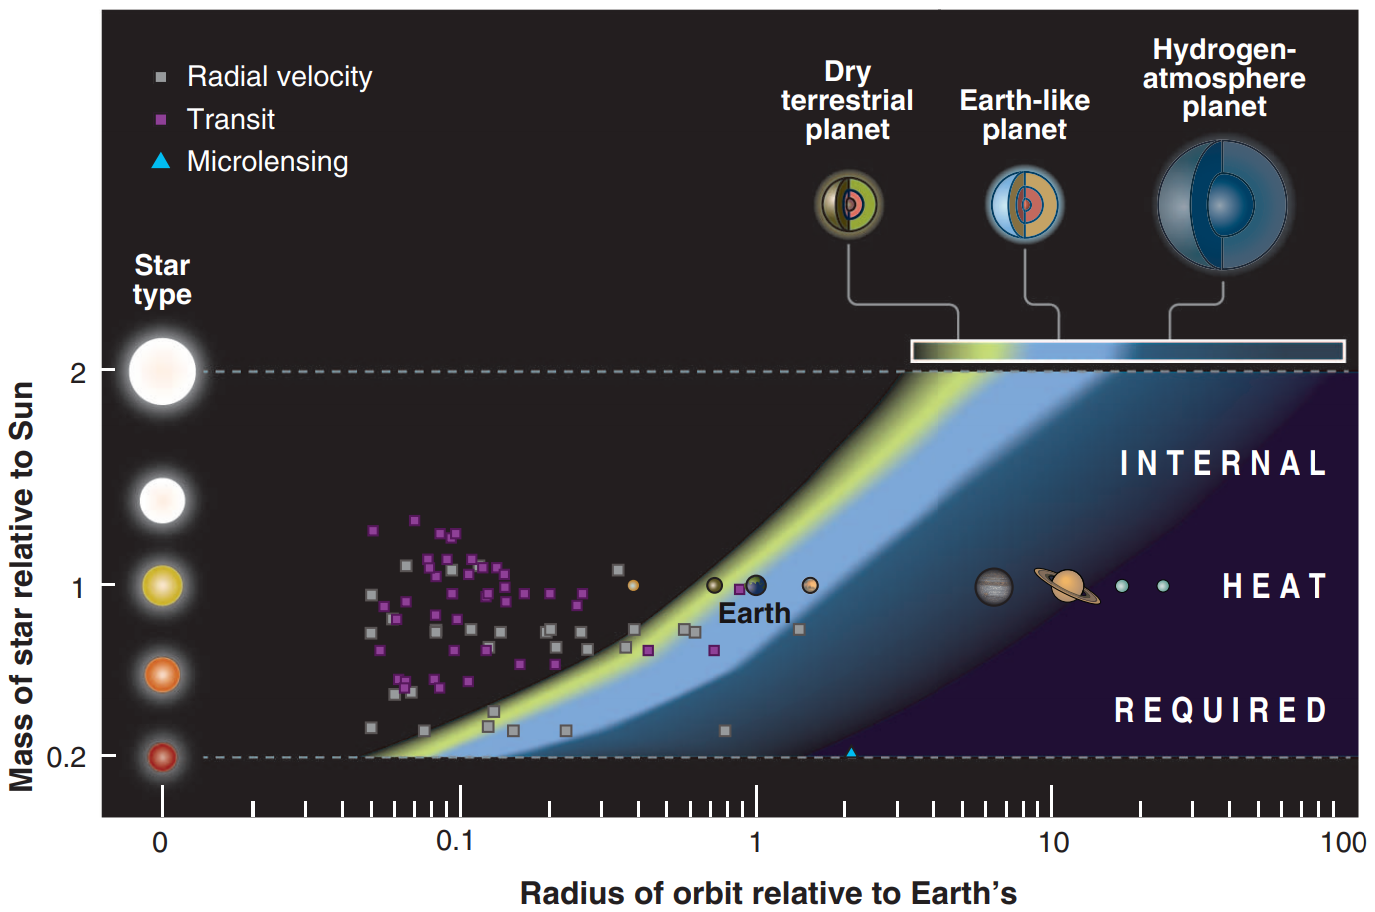
\includegraphics[width=\linewidth,]{Pic/Planets_habitability_Seager.png}\\
\begin{center}
Image taken from \cite{seager2013exoplanet}
\end{center}

\end{columns}
\end{frame}


\subsection{Stars Feature}

\begin{frame}
\frametitle{Theoretical background - Star features }
\begin{columns}
\column{0.4\textwidth}
\begin{itemize}
\item \textbf{Main features}: For this work the main features of star are the stellar luminosity (S\_L), its temperature (S\_T) and spectral type (S\_S\_T)
\item\textbf{H-R diagram}: with these features the Hertzsprung-Russell diagram classify the stars (the temperature and spectral type of a star are two faces of the same medal)
\end{itemize}
\column{0.45\textwidth}
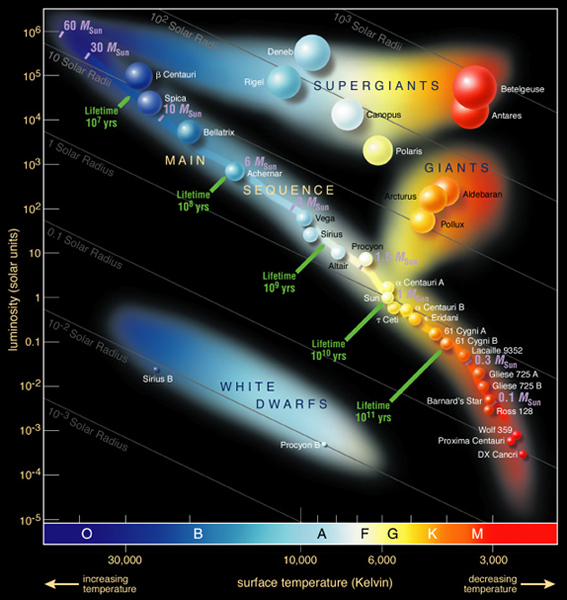
\includegraphics[width=\linewidth,]{Pic/S_T_T_explanation.png}
\begin{center}
Image taken from \cite{HR_diagram}
\end{center}
\end{columns}
\end{frame}

\subsection{Planet Features}

\begin{frame}
\frametitle{Theoretical background - Planet features }
\begin{center}
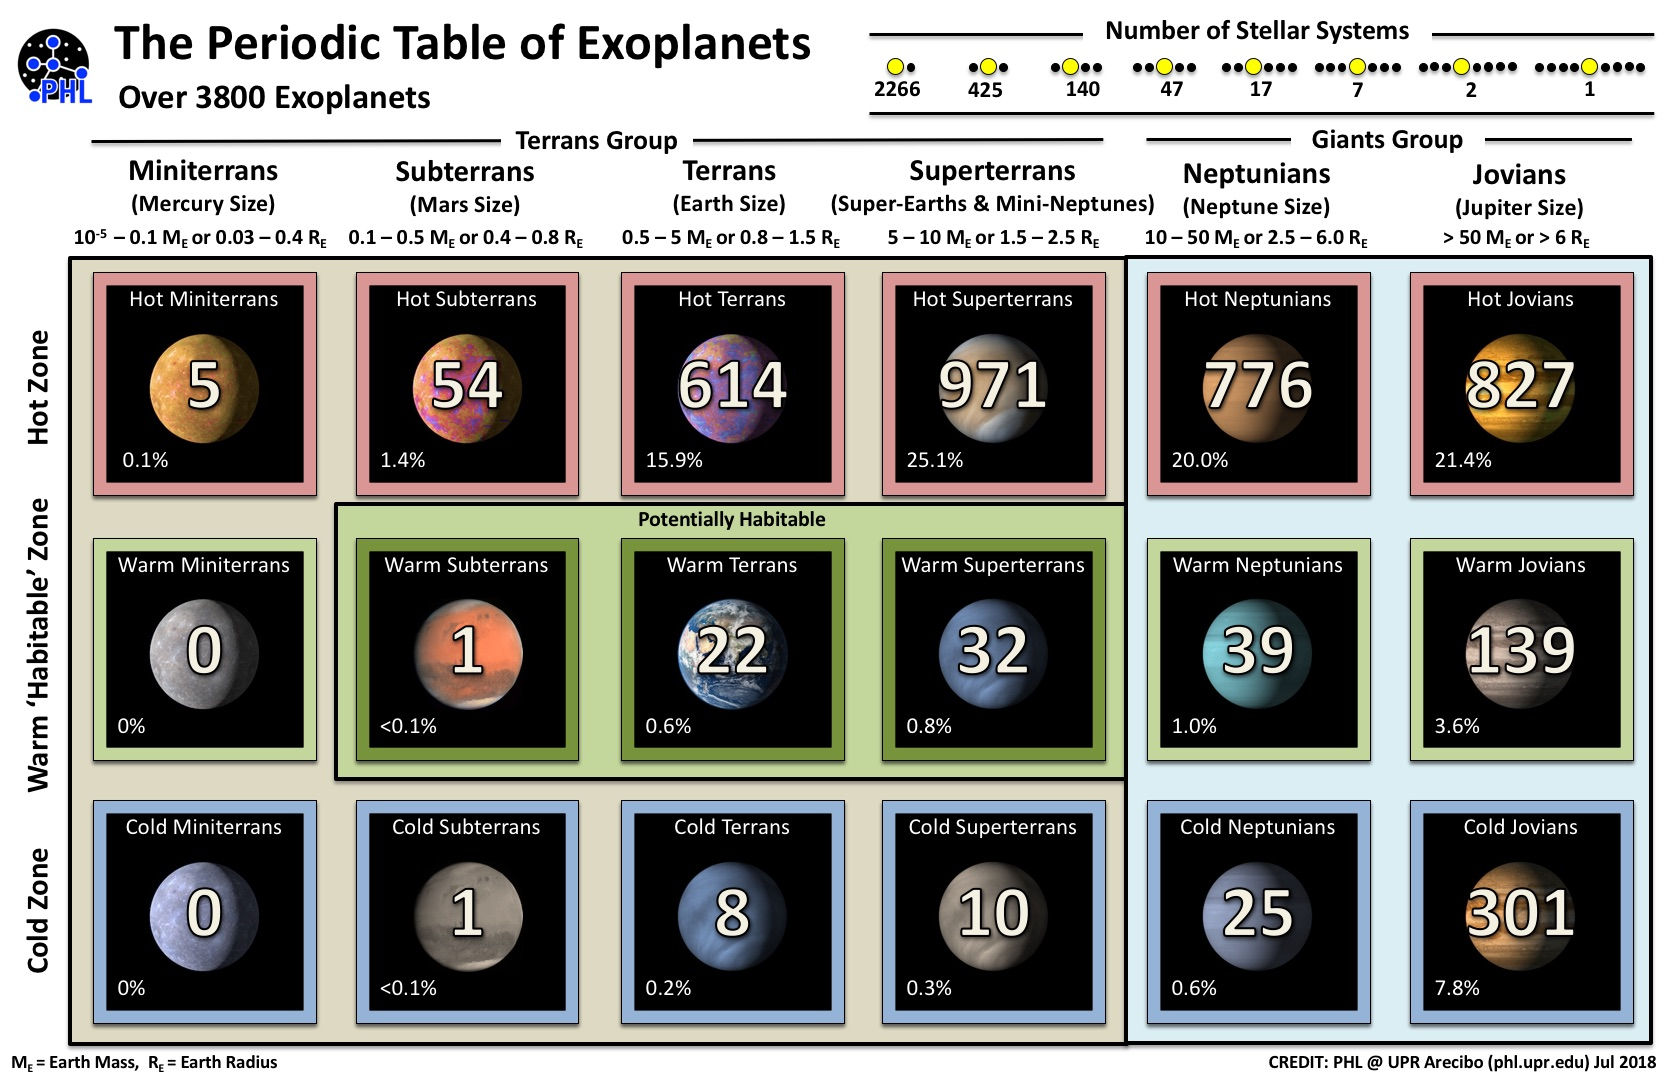
\includegraphics[width=.9\linewidth,]{Pic/PT_Confirmed.jpg}
\end{center}
\begin{center}
Image taken from \cite{exoplanets-catalog}
\end{center}
\end{frame}


\begin{frame}
\frametitle{Theoretical background - Planet features }
\begin{itemize}
\item\textbf{Distance}: in this work the mean planet distance from the host star (P\_D), the periastron (P\_PN) and the apastron (P\_A) as well the termal effective distance (P\_D\_E) from the host star  were considered. These quantities constrain the planet orbital period (P\_P) via the 3$^{th}$ Kepler law (a corollary of Newton's law of universal gravitation)
\item\textbf{Mass and Radius}: the (estimated) planet mass (P\_M) and its radius (P\_R) were considered (these are also useful to distinguish the super-earth planets) 
\item\textbf{Temperature}: the planet equilibrium temperature (P\_T\_E) defined according to the expression $T_{eq}=T_{star}\sqrt{R/2a}\left(1-A\right)^{0.25}$) where R is the star radius (S\_R), a the planet mean distance (P\_D) and A the albedo here considered as 0.3 was considered as well the planet mean stellar flux $P_F$ 
\item\textbf{Habitability}: The planet habitability was classified with a boolean variable using the values reported in the dataset \cite{planet_dataset}

\end{itemize}
\end{frame}


\section{Data inspection}
\subsection{Densities}
\begin{frame}
\frametitle{Data inspection - densities}
\begin{columns}[t]
        \column{.25\textwidth}
        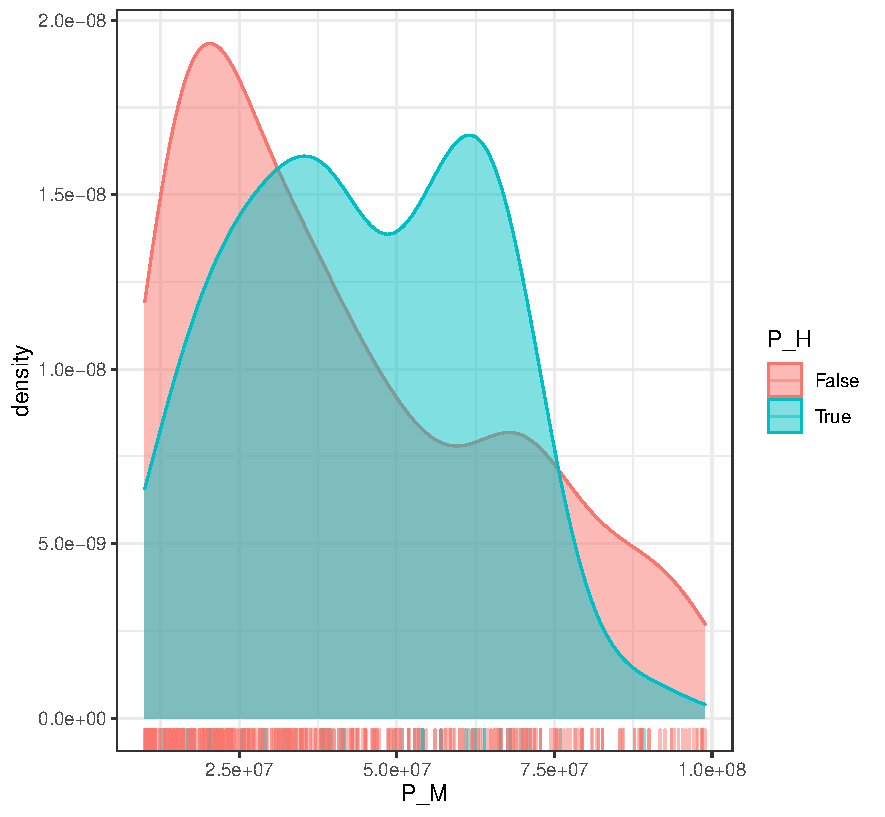
\includegraphics[width=\linewidth]{Pic/Density/P_M.pdf}
        \begin{center}
        Planet mass\\
        \end{center}
        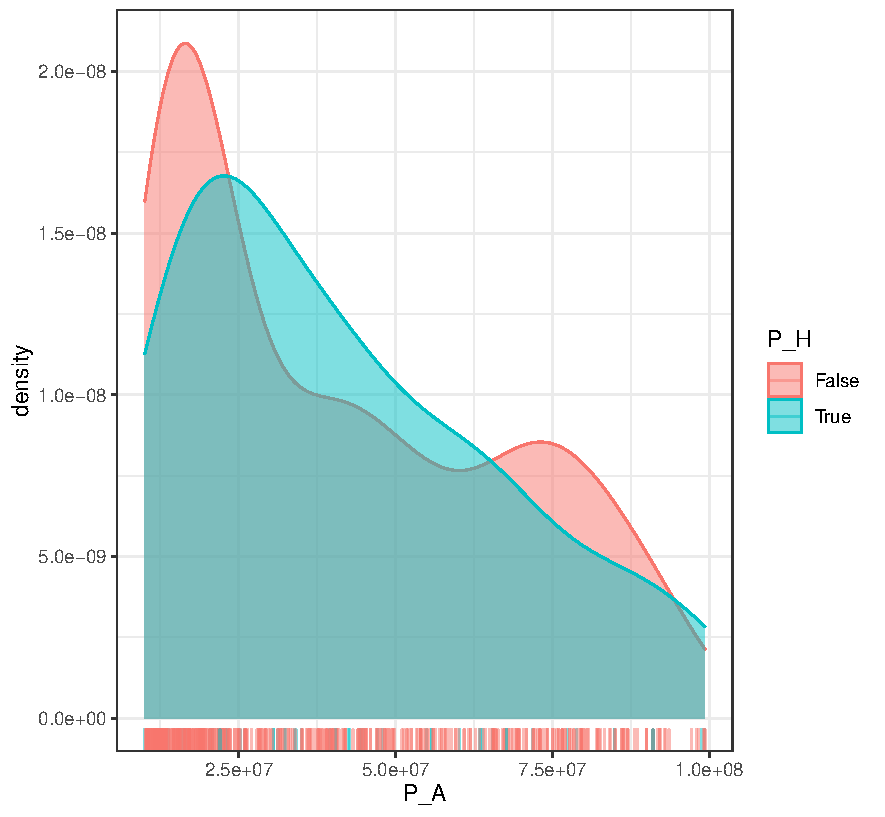
\includegraphics[width=\linewidth]{Pic/Density/P_A.pdf}
        \begin{center}
        Planet apastron\\
        \end{center}
        \column{.25\textwidth}
        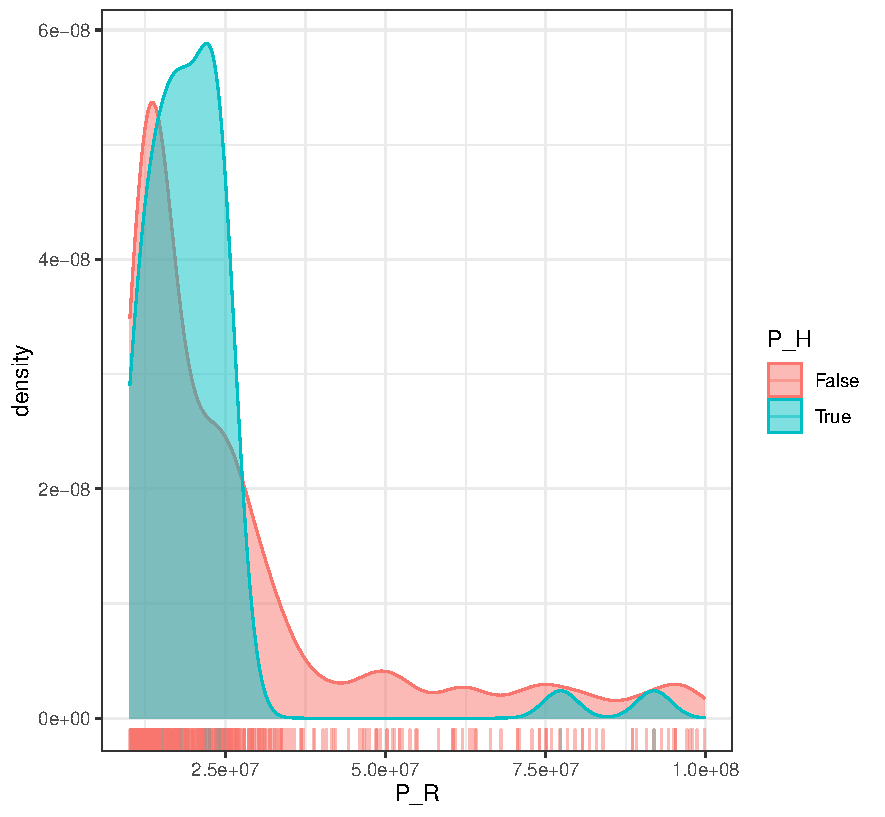
\includegraphics[width=\linewidth]{Pic/Density/P_R.pdf}
        \begin{center}
        Planet radius\\
        \end{center}
        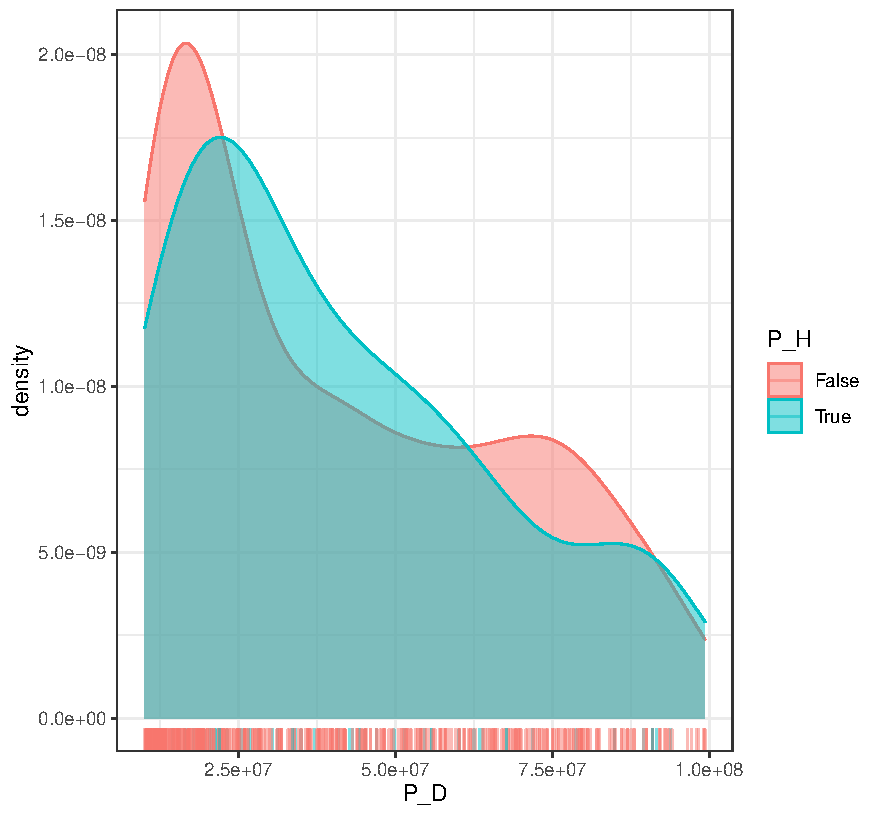
\includegraphics[width=\linewidth]{Pic/Density/P_D.pdf}
        \begin{center}
        Planet distance\\
        \end{center}
        \column{.25\textwidth}
        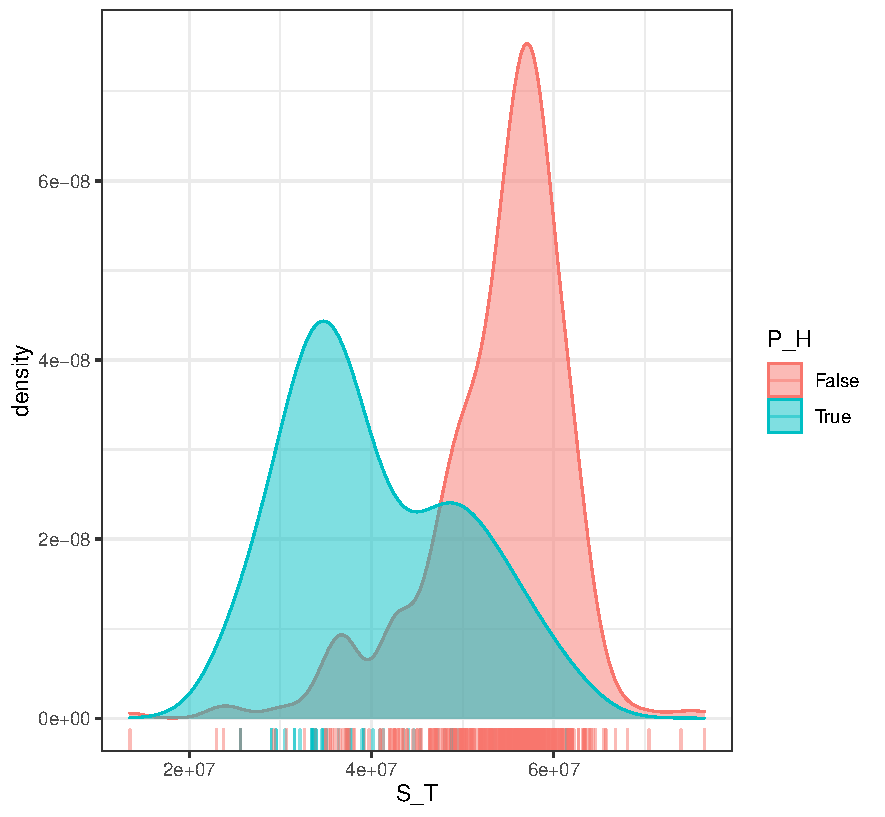
\includegraphics[width=\linewidth]{Pic/Density/S_T.pdf}
        \begin{center}
        Stellar T \\
        \end{center}
        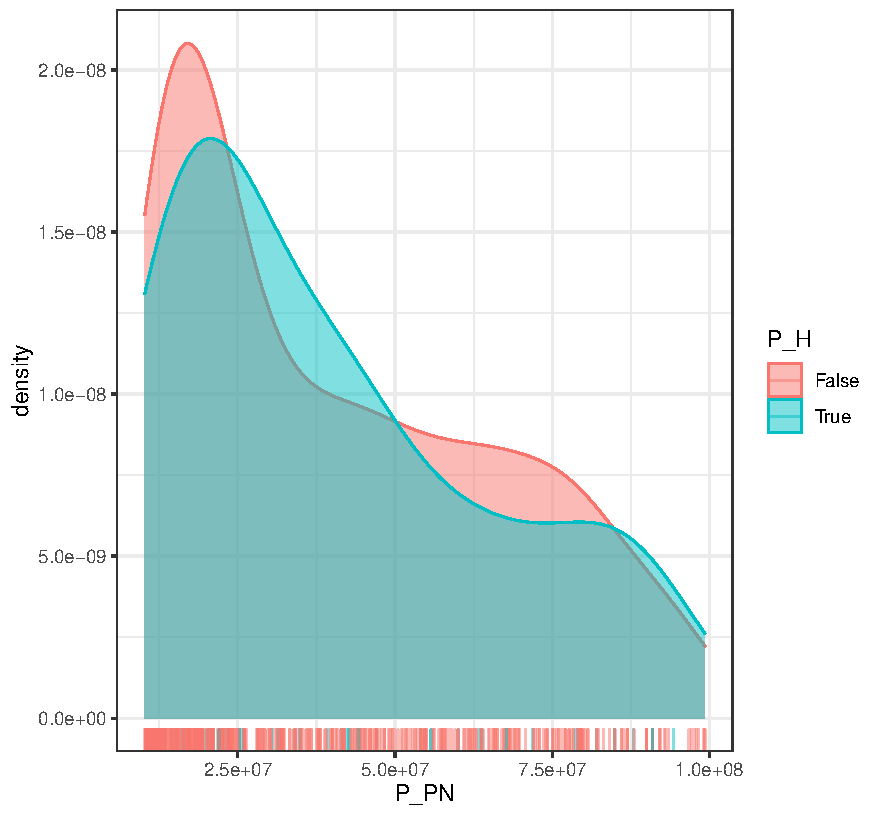
\includegraphics[width=\linewidth]{Pic/Density/P_PN.pdf}
        \begin{center}
        Planet periastron\\
        \end{center}
        \column{.25\textwidth}
        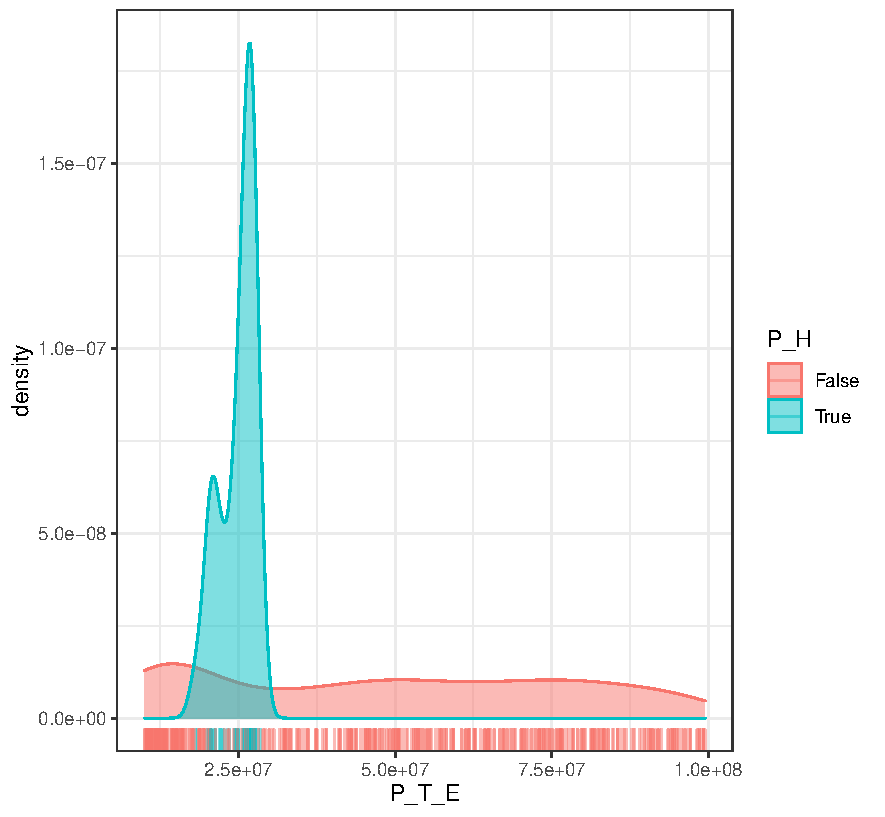
\includegraphics[width=\linewidth]{Pic/Density/P_T_E.pdf}
        \begin{center}
        P T E\\
        \end{center}
        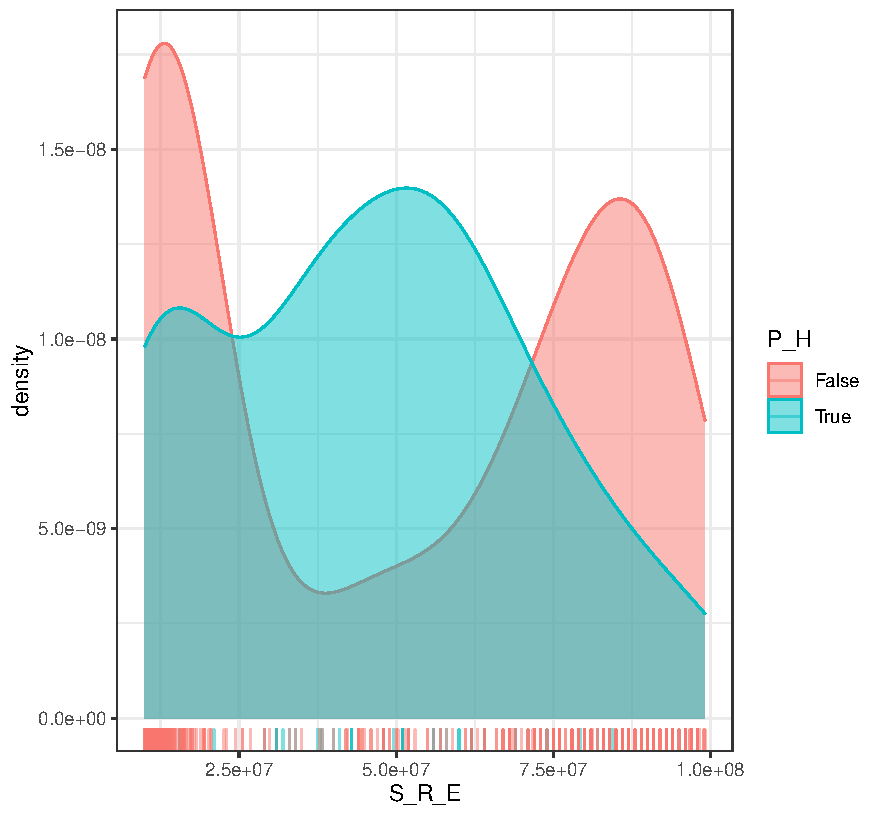
\includegraphics[width=\linewidth]{Pic/Density/S_R_E.pdf}
        \begin{center}
        Star radius\\
        \end{center}
    \end{columns}
\end{frame}

\subsection{FAMD}
\begin{frame}
\frametitle{Data inspection - FAMD}
\begin{columns}
\column{0.5\textwidth}
\begin{center}
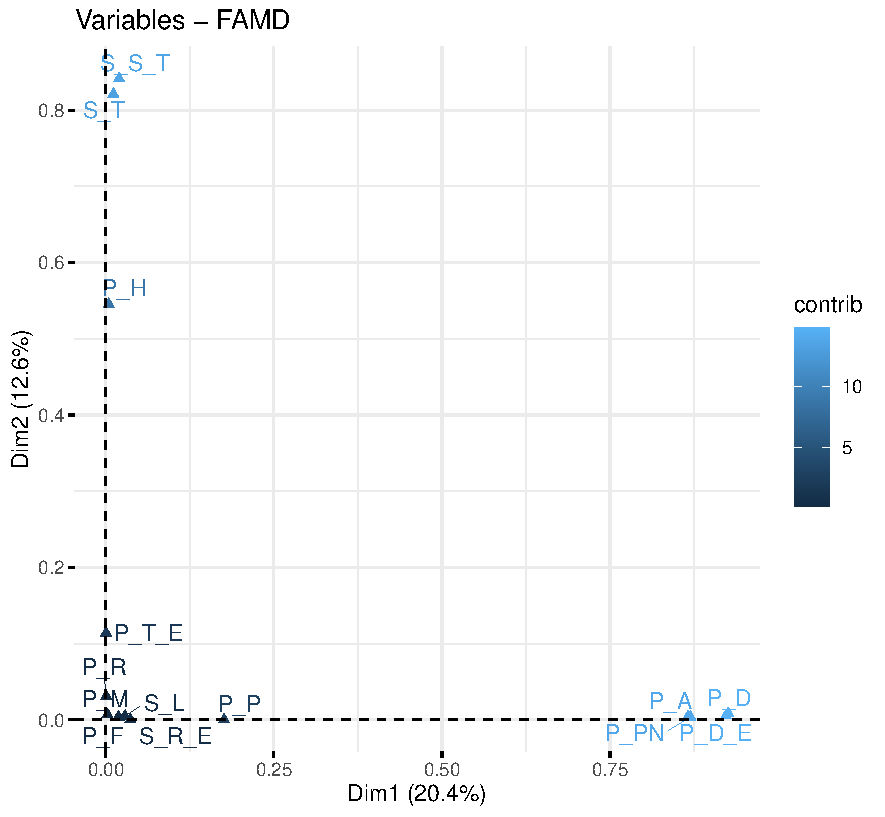
\includegraphics[width=\linewidth]{Pic/FAMD_squared_loadings.pdf}
\end{center}
\column{0.5\textwidth}
\begin{center}
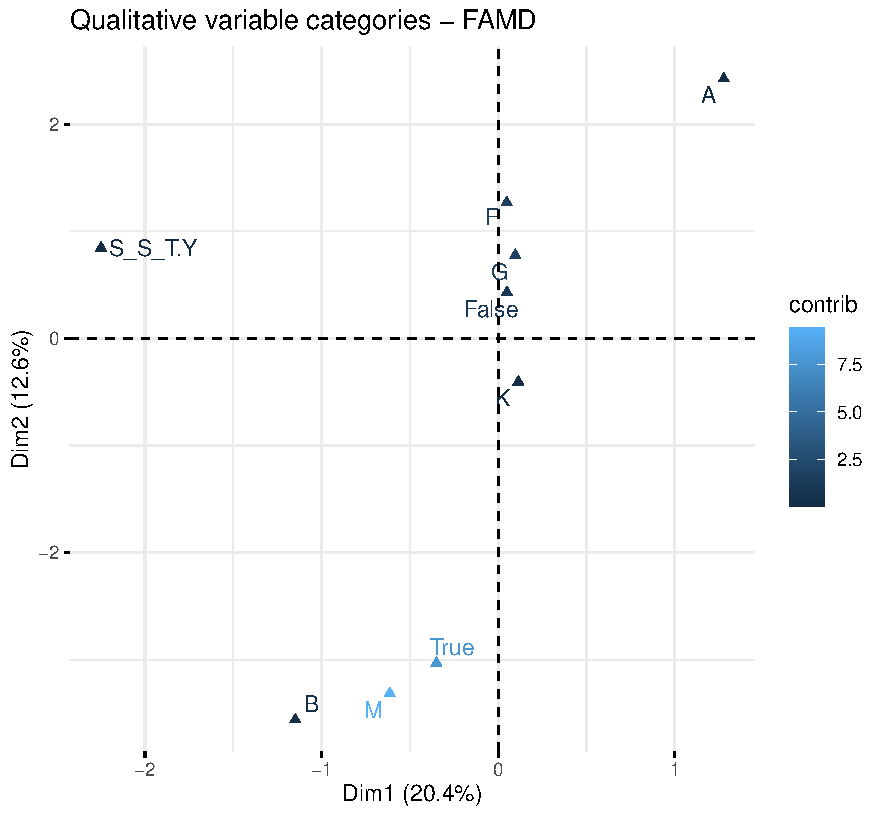
\includegraphics[width=0.7\linewidth]{Pic/FAMD_Qualitative_VAR.pdf}
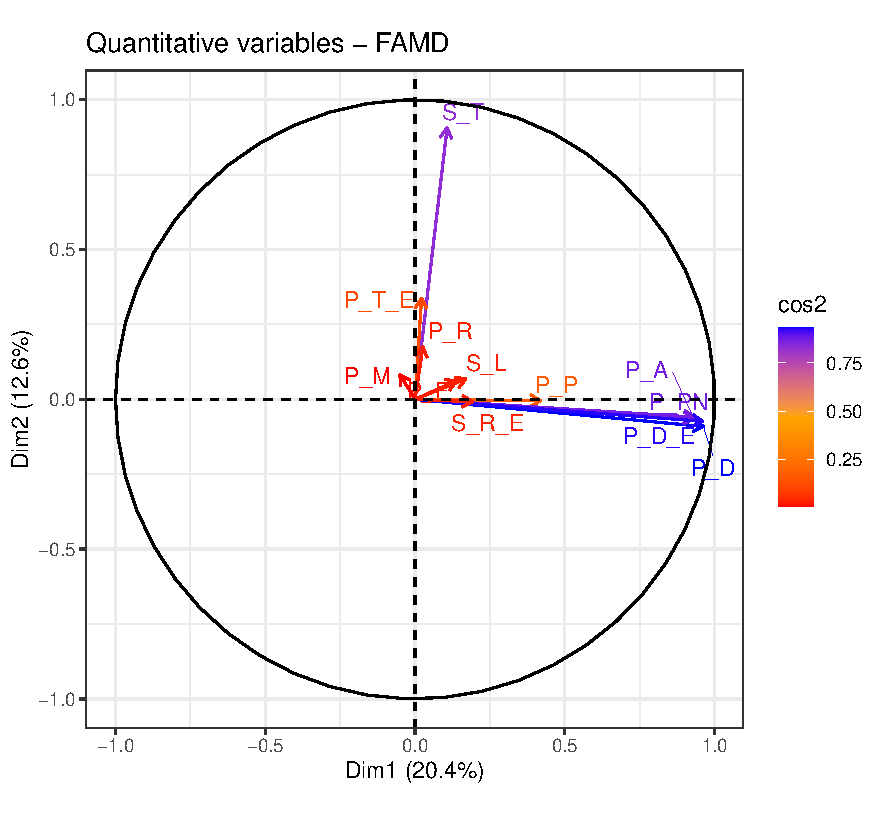
\includegraphics[width=0.7\linewidth]{Pic/FAMD_quantitative_variables.pdf}
\end{center}
\end{columns}
\end{frame}





\begin{frame}[t,allowframebreaks]
\frametitle{References}
\printbibliography
\end{frame}

\end{document}